\section{Research}\label{research}

The primary research question of this thesis is:

\textit{How to implement a transformation from typechecked Meta-Casanova(MC) in executable code?}

Where the transformation must satisfy these requirements:
\begin{enumerate}
    \item The backend must in no case produce an incorrect program.
    \item The executable must be able to inter-operate with .NET.
    \item The generated code must run on all the platforms .NET runs on.
    \item The performance of the generated program should be comparable to Python.
\end{enumerate}


The correctness requirement exists because the compiler must be reliable.
Any program can at most be as reliable as the compiler used to generate it.
\label{whydotnet}
The .NET requirement exists because of the need for a large library and inter-operability with Unity game engine.
This is because the main area of research of the organization is game-related\footnote{see section~\ref{motive}}.
The multiplatform requirement is because the games are produced for any platform.
The performance requirement is there because games have to be fast.

In order to answer the research question, seven subquestions were formulated.

\begin{enumerate}
    \item In what language should the code generator produce its output?
    \item What should the interface be between the front-end and the back-end?
    \item What should the intermediate representation of the functions be?
    \item How does the interface map to the output language?
    \item How to generate names so that they comply with the output language?
    \item How to validate the code-generator?
    \item How to validate the test programs?
\end{enumerate}

Each answer of a subquestion is provided evidence by implementing a part of the backend. 
This will in turn provide evidence to answer the main research question.

To illustrate how the different parts of the back-end relate to each other, here is a diagram of the dataflow through the backend.

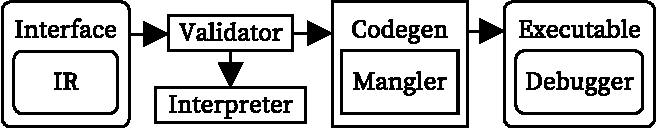
\includegraphics[width=\columnwidth]{overview}

As you can see, the front-end interface contains the Intermediate Representation (IR) and goes through the validator.
From there, depending on the compiler flags, it either goes to the interpreter or the codegen.
In case it goes to the interpreter, the program is directly executed.
In case it goes to the codegen, it is translated to the output language.
To translate all the identifiers, the mangler is needed.
The debugger is optionally embedded in the executable, depending on compiler flags.

